\documentclass[a4paper,12pt]{article}
\usepackage[utf8]{inputenc}
\usepackage[T2A]{fontenc}
\usepackage[english,russian]{babel}
\usepackage{natbib}
\usepackage{graphicx}
\usepackage{amsmath}
\usepackage{pgfplots}
\usepackage{color} %% это для отображения цвета в коде
\usepackage{listings} %% собственно, это и есть пакет listings
\usepackage{caption}
\DeclareCaptionFont{white}{\color{white}} %% это сделает текст заголовка белым
%% код ниже нарисует серую рамочку вокруг заголовка кода.
\DeclareCaptionFormat{listing}{\colorbox{white}{\parbox{\textwidth}{#1#2#3}}}
\captionsetup[lstlisting]{format=listing,labelfont=black,textfont=black}

\definecolor{bluekeywords}{rgb}{0,0,175}
\definecolor{greencomments}{rgb}{0,0.5,0}
\definecolor{redstrings}{rgb}{0.64,0.08,0.08}
\definecolor{xmlcomments}{rgb}{0.5,0.5,0.5}
\definecolor{types}{rgb}{0.17,0.57,0.68}

\lstset{ %
language=Java,                 % выбор языка для подсветки
basicstyle=\small\sffamily, % размер и начертание шрифта для подсветки кода
numbers=left,               % где поставить нумерацию строк (слева\справа)
numberstyle=\tiny,           % размер шрифта для номеров строк
stepnumber=1,                   % размер шага между двумя номерами строк
numbersep=5pt,                % как далеко отстоят номера строк от подсвечиваемого кода
backgroundcolor=\color{white}, % цвет фона подсветки - используем \usepackage{color}
showspaces=false,            % показывать или нет пробелы специальными отступами
showstringspaces=false,      % показывать или нет пробелы в строках
showtabs=false,             % показывать или нет табуляцию в строках
frame=single,              % рисовать рамку вокруг кода
tabsize=1,                 % размер табуляции по умолчанию равен 2 пробелам
captionpos=t,              % позиция заголовка вверху [t] или внизу [b] 
breaklines=true,           % автоматически переносить строки (да\нет)
breakatwhitespace=false, % переносить строки только если есть пробел
escapeinside={\%*}{*)},  % если нужно добавить комментарии в коде
commentstyle=\color{greencomments},
morekeywords={partial, var, value, get, set},
keywordstyle=\color{bluekeywords}\bfseries,
stringstyle=\color{redstrings}
}

\title{Министерство образования Российской Федерации
Московский Государственный Технический Университет им. Н.Э. Баумана}
\author{Ирина Горохова}
\date{Москва, 2017}

%%%%%%%%%%%%%%%%%%%%%%%%%%%%%%%%%%%%%%%%%%%%%%%%%%%%%%%%%%%%%%%%%%%%%%%%%%%%%%%%%%%%%%%%%%%%%%%

\begin{document}

\thispagestyle{empty}

\begin{figure}[th]
\noindent\centering{
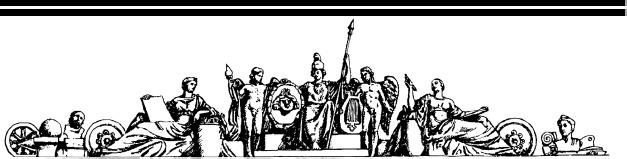
\includegraphics[scale = 0.6]{img-AFYrS7.jpg}}
\end{figure}

\begin{center}
    {\Large Министерство образования Российской Федерации\\
Московский Государственный Технический\\ Университет им. Н.Э. Баумана \\[66pt]
Отчет по лабораторной работе №7 \\
По курсу «Анализ алгоритмов»}
\end{center}

\begin{center}
    {\LARGE \textbf{Тема: «Муравьиный алгоритм»\\[90pt]}}
\end{center}

\begin{flushright}
Студент: {\bfГорохова И.Б.}\\ Группа: {\bfИУ7-51}\\[20pt] 
Преподаватель: {\bfВолкова Л.Л.}\\[80pt]
\end{flushright}

\begin{center}
    {\Large Москва, 2017}
\end{center}

\newpage

\tableofcontents
%%%%%%%%%%%%%%%%%%%%%%%%%%%%%%%%%%%%%%%%%%%%%%%%%%%%%%%%%%%%%%%%%%%%%%%%%%%%%%%%%%%%5
\newpage
\section*{Постановка задачи}
\addcontentsline{toc}{section}{Постановка задачи}
В ходе лабораторной работы предстоит:
\begin{enumerate}
    \item реализовать муравьиный алгоритм на языке программирования;
    \item сравнить работу алгоритма при разных значениях параметров, задающих веса феромона и времени жизни колонны.
\end{enumerate}
%%%%%%%%%%%%%%%%%%%%%%%%%%%%%%%%%%%%%%%%%%%%%%%%%%%%%%%%%%%%%%%%%%%%%%%%%%%%%%%%%%%
\section*{Реализация}
\addcontentsline{toc}{section}{Реализация}
\subsection*{Суть алгоритма}
\addcontentsline{toc}{subsection}{Суть алгоритма}

Муравьиный алгоритм (алгоритм оптимизации подражанием муравьиной колонии) — один из эффективных алгоритмов для нахождения приближённых решений задачи коммивояжёра, а также решения аналогичных задач поиска маршрутов на графах. \\

Суть подхода заключается в анализе и использовании модели поведения муравьёв, ищущих пути от колонии к источнику питания и представляет собой метаэвристическую оптимизацию.\\

Моделирование поведения муравьев связано с распределением феромона на тропе — ребре графа в задаче коммивояжера. При этом вероятность включения ребра в маршрут отдельного муравья пропорциональна количеству феромона на этом ребре, а количество откладываемого феромона пропорционально длине маршрута. Чем короче маршрут, тем больше феромона будет отложено на его ребрах, следовательно, большее количество муравьев будет включать его в синтез собственных маршрутов.\\

\addcontentsline{toc}{subsection}{Программная реализация алгоритма}
\subsection*{Программная реализация алгоритма}


Для реализации муравьиного алгоритма на языке Java были написаны класс Ant, приведенный в листинге 1, и несколько методов, представленных в листингах .......
Граф,описывающий города и дороги между ними, в программе представлен симметричной относительно главной диагонали матрицей смежности размером N*N, где N - количество городов (вершин графа), (i,j)-й элемент которой равен длине пути из i-той вершины в j-тую (весу ребра/дуги).
\begin{lstlisting}[label=some-code,caption=Класс Ant]
private class Ant {
    public int tour[] = new int[graph.length];
    public boolean visited[] = new boolean[graph.length];

    public void visitTown(int town) {
        tour[currInd + 1] = town;
        visited[town] = true;
    }

    public boolean isVisited(int i) {
        return visited[i];
    }

    public int tourLength() {
        int length = graph[tour[townsN - 1]][tour[0]];
        for (int i = 0; i < townsN - 1; i++) {
            length += graph[tour[i]][tour[i + 1]];
        }
        return length;
    }

    public void clear() {
        for (int i = 0; i < townsN; i++)
            visited[i] = false;
    }
}
\end{lstlisting}
{\bf Поля класса Ant:}
\begin{itemize}
    \item tour - массив целых чисел, представляющий собой путь муравья, где каждый элемент массива - номер посещенного города ($graph.length$ - количество городов, $graph$ - матрица весов);
    \item visited - массив флагов, где i-тый элемент равен $true$, если муравей уже посетил i - тый город и $false$ - если еще не посетил.
\end{itemize}
{\bf Методы класса Ant:}
\begin{itemize}
    \item visitTown() - добавляет в массив с путём муравья номер города $town$ и помечает этот город как посещённый этим муравьем;
    \item isVisited() - возвращает $true$, если муравей уже был в городе с номером i, и $false$ - иначе;
    \item tourLength() - суммирует расстрояния из одного города в другой по пути муравья и возвращает значение длины полного пути;
    \item clear() - отчищает массив с флагами посещенных городов.
\end{itemize}

В главном классе AntAlgo созданы следующие поля:
\begin{lstlisting}[label=some-code,caption=Поля класса AntAlgo]
public class AntAlgo {
    private double amountOfPheromon = 1;
    private double prefPheromon = 0.5;        //alpha
    private double prefGreedy = 0.5;          //beta
    private double evaporationCoef = 0.5;     //p
    private double newPheromonCoef = 50;      //Q
    private double coefOfAntsCount = 0.8;
    
    private int townsN = 0;
    private int antsM = 0;
    
    private int graph[][] = null;
    private double pheromon[][] = null;
    private Ant ants[] = null;
    private double probs[] = null;
    
    private int currInd = 0;
    
    public int[] bestTour;
    public int bestTourLen;
    
    //...

\end{lstlisting}
\begin{itemize}
    \item amountOfPheromon - начальное значение феромона;
    \item prefPheromon - величина, определяющая «стадность» алгоритма;
    \item prefGreedy  - величина, определяющая «жадность» алгоритма;
    \item evaporationCoef - коэффициент испарения феромона;
    \item newPheromonCoef - параметр, имеющий значение порядка длины оптимального пути;
    \item coefOfAntsCount - коэффициент "муравьев на город". (Количество муравьев в колонии = количество городов * coefOfAntsCount);
    \item townsN - количество городов;
    \item antsM - количество муравьев (townsN * coefOfAntsCount);
    \item graph - матрица размерности N*N, где N = townsN, описывающая длины дорог между городами;
    \item pheromon - матрица, содержащая данные о количестве феромона на дорогах;
    \item ants - массив муравьев;
    \item probs - массив, содержащий в i-той ячейке вероятность похода муравья в i-тый город (заполняется для каждого перехода каждого муравья заново);
    \item currInd - количество уже посещенных городов, принимает значения от 0 до townsN-1;
    \item bestTour - массив, содержащий порядок лучшего на данный момент пути по длине;
    \item bestTourLen - длина пути из bestTour.
\end{itemize}

Главным методом, находящим кратчайший путь, является метод $solve()$. Колония муравьев ищет путь до источника питания в течение каждого момента времени жизни колонии, которое равно maxIterations, где одна итерация - один момент времени. В каждый момент времени муравьи начинают движение из рандомного города, проходят все города и возвращаются в начальный город, обновляется след феромона на дорогах и обновляется лучшее решение (кратчайший на данный момент путь).\\
Метод представлен в листинге 3, а в листинге 4 представлены методы, вызываемые из solve(). 
\begin{lstlisting}[label=some-code,caption=Метод solve()]
public void solve() {
    for (int i = 0; i < townsN; i++)
        for (int j = 0; j < townsN; j++)
            pheromon[i][j] = amountOfPheromon;

    int iteration = 0;
    int maxIterations = 50;
    while (iteration < maxIterations) {
        startAnts();
        moveAnts();
        updatePheromone();
        updateBestTour();
        iteration++;
    }
    System.out.println("Best tour length: " + bestTourLen + ". Tour: " + tourToString(bestTour));
}
\end{lstlisting}

\begin{lstlisting}[label=some-code,caption=Методы класса AntAlgo]
private void startAnts() {
    currInd = -1;
    for (Ant a: ants) {
        a.clear();
        a.visitTown(rand.nextInt(townsN));
    }
    currInd++;
}

private void moveAnts() {
    while (currInd < townsN -1) {
        for (Ant a: ants)
            a.visitTown(selectNextTown(a));
        currInd++;
    }
}

private int selectNextTown(Ant ant) {
    getProbability(ant);
    
    double r = rand.nextDouble();
    double total = 0;
    for (int i = 0; i < townsN; i++) {
        total += probs[i];
        if (total >= r)
            return i;
    }
}

private void getProbability(Ant ant) {
    int ind = ant.tour[currInd];
    
    double znam = 0.0;
    for (int i = 0; i < townsN; i++)
        if (!ant.isVisited(i))
            znam += Math.pow(pheromon[ind][i], prefPheromon) * Math.pow(1.0/graph[ind][i], prefGreedy);

    for (int i = 0; i < townsN; i++) {
        if (ant.isVisited(i))
            probs[i] = 0.0;
        else {
            double chisl = Math.pow(pheromon[ind][i], prefPheromon) * Math.pow(1.0/graph[ind][i], prefGreedy);
            probs[i] = chisl/znam;
        }
    }
}

private void updatePheromone() {
    for (int i = 0; i < townsN; i++)
        for (int j = 0; j < townsN; j++)
            pheromon[i][j] *= (1 - evaporationCoef);

    for (Ant a: ants){
        double antContribution = newPheromonCoef/a.tourLength();
        pheromon[a.tour[townsN-1]][a.tour[0]] += antContribution;
        for (int i = 0; i < townsN-1; i++) {
            pheromon[a.tour[i]][a.tour[i+1]] += antContribution;
        }
    }
}

private void updateBestTour() {
    if (bestTour == null) {
        bestTour = ants[0].tour;
        bestTourLen = ants[0].tourLength();
    }
    for (Ant a: ants) {
        if (a.tourLength() < bestTourLen) {
            System.out.println("Old: " + bestTourLen + " New: " + a.tourLength());
            bestTour = a.tour.clone();
            bestTourLen = a.tourLength();
        }
    }
}
    
\end{lstlisting}\\

startAnts() - для каждого муравья выбирается рандомный город как начальный.\\

moveAnts() - строится маршрут для каждого муравья. Города выбираются с помощью метода selectNextTown().\\

selectNextTown() - для каждого муравья заполняется массив prob, где i-тый элемент - вероятность выбора i-того города следующим к посещению. Получают рандомное число r от 0 до 1. Вероятности определяют ширину зоны для каждого из городов. город, в зону которого попадает r, и выбирается следующим для похода.\\
Пример: Пусть есть три города, которые муравей может посетить. С вероятностью 0.35 он может пойти в 1ый город, с 0.5 - во второй, с 0.15 - в третий. Зоны распределяются таким образом:[0-0.35) - 1ый город, [0.35-0.85) - 2ой город, [0.85-1] - 3ий город . Пусть рандомное число r = 0.45. Оно попадает в зону второго города, следовательно для посещения муравья выбирается второй город.\\

getProbability() - заполняется массив probs, используемый в функции selectNextTown(). Для заполнения массива используется формула (1):
\begin{equation}
    \begin{matrix}
    P_i_j_,_k(t) & = 
    & \left\{
    \begin{matrix}
    \frac{[\tau_i_j(t)]^\alpha * [\eta_i_j]^\beta}{\sum\limits_{l = J_i_,_k} [\tau_i_j(t)]^\alpha * [\eta_i_j]^\beta }   & j \in J_i_,_k \\
    0 & j \notin J_i_,_k \\
    \end{matrix} \right. 
    \end{matrix}
\end{equation}
где $\alpha, \beta$ в программе заданы, как prefPheromon и prefGreedy соответственно (величина, определяющая «стадность» алгоритма и «жадность» алгоритма); $\tau$ - feromon[i][j], а $\eta$ - $\frac{1}{graph[i][j]}$ ( матрица размерности, описывающая длины дорог между городами и матрица, содержащая данные о количестве феромона на дорогах)\\

updatePheromone() - в конце каждого похода обновляется значение феромона на дорогах, используется формула (2):
\begin{equation}
\tau_i_j(t+1) = (1-p)*\tau_i_j(t) + \Delta\tau_i_j(t); \Delta\tau_i_j(t) = \sum\limits_{k = 1}^{m} \Delta\tau_i_j_,_k(t)
\end{equation}

где 
\begin{equation}
    \begin{matrix}
    \Delta\tau_i_j_,_k(t) & = 
    & \left \{
    \begin{matrix}
    \frac{Q}{L_k(t)}, & (i,j) \in T_k(t) \\
    0, & (i,j) \notin T_k(t) \\
    \end{matrix} \right
    \end{matrix}
\end{equation}

p - коэффициент испарения феромона; Q - параметр, имеющий значение порядка длины оптимального пути; $L_k$ - длина маршруту, пройденная муравьем k к моменту времени t; m - количество муравьев в колонии.\\

updateBestTour() - для каждого муравья колонии, пройденный им маршрут в данный момент времени сравнивается с маршрутом минимальной на данный момент длины. Если найден маршрут меньшей длины, то данные о лучшем маршруте обновляются.\\

Так же для решения задачи использовались функции graphFilling() - заполнение матрицы смежностей данными, printMatrix() - печать матрицы смежностей в консоли, tourToString() - функция печати последовательности номеров городов в консоль.\\

Функция Main() выглядит следующим образом:
\begin{lstlisting}[label=some-code,caption=Точка входа в программу. Функция Main()]
public static void main(String[] args) throws IOException {
    AntAlgo algorithm = new AntAlgo();
    algorithm.graphFilling(true, 100);
    
    antsM = (int)(townsN*coefOfAntsCount);
    pheromon = new double[townsN][townsN];
    ants = new Ant[antsM];
    for (int i = 0; i < antsM; i++)
        ants[i] = new Ant();
    probs = new double[townsN];

    algorithm.printMatrix(true);
    algorithm.solve();
}
\end{lstlisting}

\section*{Эксперимент}
\addcontentsline{toc}{section}{Эксперимент}

В качестве первого эксперимента проверяется эффективность работы реализованного алгоритма в зависимости от параметров $\alpha$ $\beta$ в формуле (1). \\
\addcontentsline{toc}{subsection}{Эксперимент с значениями "стадности" и "жадности" алгоритма}
Входные данные:
\begin{itemize}
    \item количество итераций maxIterations = 100;
    \item размерность матрицы townsN = 100;
    \item $\alpha$ принимает значения от 0 до 1 с шагом 0.1 (при $\alpha$ = 0 лгоритм вырождается до жадного алгоритма (будет выбран ближайший город));
    \item $\beta$ принимает значения от 1 до 0 с шагом 0.1.
\end{itemize}
Полученные данные представлены в Таблице 1.

{\flushright Таблица 1. Результаты эксперимента 1. \par}

\begin{center}
\begin{tabular}{|c|c|c|}
\hline
\alpha & \beta & Длина найденного\\
& & кратчайшего маршрута\\
\hline
\hline
0.0 & 1.0 &  413 \\
0.1 & 0.9 &  401 \\
0.2 & 0.8 &  345 \\
0.3 & 0.7 &  343 \\
0.4 & 0.6 &  309 \\
0.5 & 0.5 &  309 \\
0.6 & 0.4 &  304 \\
0.7 & 0.3 &  304 \\
0.8 & 0.2 &  304 \\
0.9 & 0.1 &  304 \\
1.0 & 0.0 &  304 \\
\hline
\end{tabular}
\end{center}

\addcontentsline{toc}{subsection}{Эксперимент с значениями времени жизни колонии}
В качестве второго эксперимента проверяется эффектривность работы реализованного алгоритма в зависимости от количества итераций (времени жизни колонии муравьев).\\
Входные данные: 
\begin{itemize}
    \item $\alpha$ = 0.5;
    \item $\beta$ = 0.5;
    \item размерность матрицы townsN = 50;
    \item количество итераций maxIterations (время жизни колонии) принимает значение от 100 до 1000 с шагом 100.
\end{itemize}

Полученные данные приведены в Таблице 2.
{\flushright Таблица 2. Результаты эксперимента 2. \par}

\begin{center}
\begin{tabular}{|c|c|}
\hline
Время жизни & Длина найденного\\
колонии & кратчайшего маршрута\\
\hline
\hline
 100 & 425\\
 200 & 409\\
 300 & 409\\
 400 & 408\\ 
 500 & 388\\
 600 & 388\\
 700 & 385\\
 800 & 384\\
 900 & 377\\
1000 & 377\\
\hline
\end{tabular}
\end{center}

\addcontentsline{toc}{subsection}{Выводы из эксперимента}
\subsection*{Выводы из эксперимента}

По результатам исследования результатов муравьиного алгоритма на разных значениях "жадности" и "стадности" можно прийти в выводу, о том, что эффективность повышается в случае увеличения коэффициента "жадности" (при $\alpha$ = 0 муравей просто будет выбирать призжайший к нему непосещенный город). Так же можно сделать вывод, что выбор $\alpha$ = 0.5 и больше ($\beta$ = 0.5 и меньше соответственно) несущественно будет влиять на результат работы алгоритма.\\
По результатам эксперимента с поиском кратчайшего маршрута с разным временем жизни колонии муравьев подтвердилось предположение, о том, что более точный результат может быть получен на большом количестве итераций (времени жизни колонии муравьев).

\addcontentsline{toc}{section}{Заключение}
\section*{Заключение}

В ходе лабораторной работы я реализовала муравьиный алгоритм на языке программирования Java и провела сравнение работы алгоритма при разных значениях параметров, задающих веса феромона и времени жизни колонны.

\end{document}
